\documentclass{article}

\usepackage[printqrbox=false,printhint=false,printanswer=true,printmarkingguide=false,printdraftpaper=false]{unswalgos}

\usepackage{tikz}
\usetikzlibrary{patterns}
\usetikzlibrary{shapes,fit}
\usepackage{tkz-fct}
\usepackage{wrapfig}
\usepackage{subfig}

\usepackage{mathtools}
\usepackage{amssymb}
\usepackage{booktabs,multicol,multirow}
\usepackage{wasysym}
\usepackage{tcolorbox}

\DeclareMathOperator*{\argmax}{arg\,max}
\DeclareMathOperator*{\argmin}{arg\,min}
\DeclareMathOperator{\NAND}{NAND}
\DeclareMathOperator{\AND}{AND}
\DeclareMathOperator{\OR}{OR}
\DeclareMathOperator{\NOT}{NOT}

\usepackage{xspace}

\fancyfoot[L]{\leftmark}
\fancyfoot[R]{\rightmark}

\usepackage{graphicx}
\usepackage{float}
\usepackage{subfigure}

\usepackage{framed}
% This enables new paragraphs without indentation
\usepackage[parfill]{parskip}

\newcommand{\sem}{22T2}
\newcommand{\semester}{Term 2, 2022}
\SubjectNo{COMP3151}
\newcommand{\taskname}{Homework 8}
\Institution{Jinghan Wang, z5286124} % Replace this with your name and zID


\begin{document}

\setcounter{question}{0}

\begin{Question} [\large\textbf {The Byzantine Generals Algorithm{[6 marks]}}]
    In the Byzantine Generals Algorithm, suppose that there is exactly 1 (one) traitor and that Ivan's data structures are:
    \begin{figure}[H]
        \centering 
        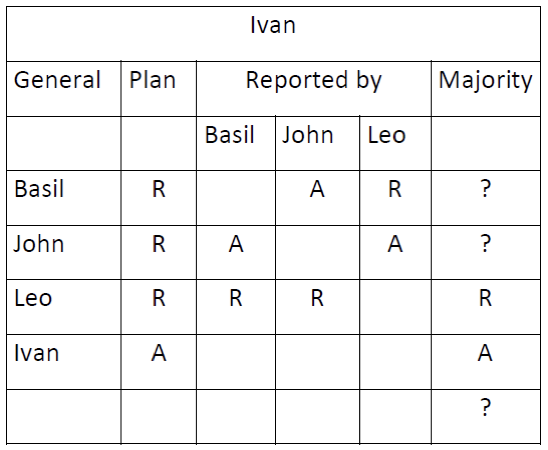
\includegraphics[width=s\textwidth]{DV_demand1}
    \end{figure}

\begin{Subquestion}
    Who is the traitor? Justify your answer (explain why this general is the traitor and why none of the other generals can be the traitor).
    
\begin{answer}
    Answer:
    \begin{quote}
        
    \end{quote}
\end{answer}
\end{Subquestion}


\begin{Subquestion}
    What does Ivan decide about Basil's and John's plans? What does Ivan decide about the overall majority plan?
    
\begin{answer}
    Answer:
    \begin{quote}
        
    \end{quote}
\end{answer}
\end{Subquestion}

\begin{Subquestion}
    Using DAJ, construct a minimal scenario leading to the shown data structure for Ivan. In this minimal scenario, the traitor's only incorrect messages should be the ones in Ivan's data structure above. Provide a screenshot of the main window in DAJ.
    
\begin{answer}
    Answer:
    \begin{quote}
        
    \end{quote}
\end{answer}
\end{Subquestion}

\begin{Subquestion}
    For the scenario constructed in the previous question, provide screenshots of the $4$ (four) knowledge trees that DAJ constructs about each of the generals. Note that knowledge trees are called "message trees" in DAJ. Which of these knowledge (message) trees indicate the traitor's incorrect messages?
    
\begin{answer}
    Answer:
    \begin{quote}
        
    \end{quote}
\end{answer}
\end{Subquestion}
\end{Question}


\clearpage
\setcounter{question}{1}

\begin{Question} [\large\textbf {The Dijkstra-Scholten Algorithm{[4 marks]}}]
    A distributed system with $4$ (four) nodes including $1$ (one) environment node is depicted with the following directed graph:
\begin{figure}[H]
    \centering 
    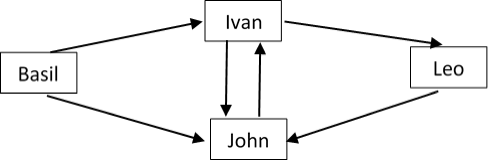
\includegraphics[width=0.9\textwidth]{DV_demand2}
\end{figure}
Using DAJ, construct a scenario for each of the $4$ (four) different spanning trees in the above directed graph. These scenarios differ in the order of the sent messages (but note that some orders of sent messages result in the same spanning tree, while you have to find all different spanning trees). For each of these scenarios, only provide a screenshot of the spanning tree that DAJ constructs.
    
\begin{answer}
    Answer:
    \begin{quote}
        
    \end{quote}
\end{answer}
\end{Question}


\clearpage
\setcounter{question}{2}

\begin{Question} [\large\textbf {Permissionless consensus{[3 marks]}}]
    Bitcoin uses what's called \textit{proof-of-work} consensus, where the first node to solve a computationally expensive puzzle gets to pick the next block.

    How does Bitcoin mitigate the problem of two nodes solving the puzzle at roughly the same time, causing a split decision? Skim the Bitcoin white paper for the answer. Explain informally and in your own words.

\begin{answer}
    Answer:
    \begin{quote}
        
    \end{quote}
\end{answer}
\end{Question}


\end{document}